% ju 06-Jun-22
\documentclass[a4paper,12pt,fleqn,parskip=half]{scrartcl}
\usepackage[ngerman]{babel}
\usepackage[utf8]{inputenc}
\usepackage[T1]{fontenc}

% Schrift
%\usepackage{lmodern}
\usepackage[osf,sc]{mathpazo} 
\usepackage[scale=.9,semibold]{sourcecodepro}   
\usepackage[osf]{sourcesanspro}  

\usepackage[headsepline]{scrlayer-scrpage}
\pagestyle{scrheadings}
\clearpairofpagestyles

\usepackage[table,dvipsnames,usenames]{xcolor}
\usepackage{textcase}
\usepackage{nameref}
\usepackage{hyperref}
\usepackage{tabularx}
\usepackage{multirow}
\usepackage{multicol}
\usepackage{caption, booktabs}
\usepackage{graphicx} 
\usepackage{scrhack}    
\usepackage{url}%% Links
\usepackage[inline]{enumitem}
\usepackage{pifont}
\usepackage{eurosym}% \euro 20,-
\usepackage{amsmath}
\usepackage{amsfonts}
\usepackage{amssymb}
\usepackage{array}            % Extending the array and tabular environments
\usepackage{chngcntr}         % Change the resetting of counters
\usepackage[version=4]{mhchem}
\usepackage{stmaryrd}
\usepackage{siunitx}
\usepackage{float}
\usepackage{csquotes}
\usepackage{subcaption}
\usepackage{mathtools}
\usepackage{icomma}%Dezimaltrennzeichen
\usepackage{multimedia}%Video: \movie[externalviewer]{(video.mov)}{video.mov}
\usepackage{epstopdf}
\usepackage{footnote}
\usepackage{qrcode}% Anwendung: \qrcode[hyperlink,level=Q,version=2,height=1cm]{\website}
\usepackage{underscore}% Unterstrich ____

% PDF Dokumente einbinden
\usepackage{pdfpages}% \includepdf[pages=-]{Tabellen/Excel.pdf}
\RequirePackage{lastpage}  % Pagecounter

\addto\captionsngerman{%
\renewcommand{\figurename}{Abb.}
\renewcommand{\tablename}{Tab.}
}

% listings
\usepackage{listings}
\lstset{basicstyle=\linespread{1}\ttfamily\small,floatplacement=!htb,captionpos=t,abovecaptionskip=.5\baselineskip,belowcaptionskip=.5\baselineskip,upquote=true,showstringspaces=false,inputencoding=utf8,tabsize=4,
    	keywordstyle=\bfseries ,
	commentstyle=\color{rot5},
	stringstyle=\color{orange},
	breaklines=true,
  	postbreak=\mbox{\textcolor{black}{$\hookrightarrow$}\space},
	breakatwhitespace=false
}
\lstset{literate={á}{{\'a}}1 {é}{{\'e}}1 {í}{{\'i}}1 {ó}{{\'o}}1 {ú}{{\'u}}1 {Á}{{\'A}}1 {É}{{\'E}}1 {Í}{{\'I}}1 {Ó}{{\'O}}1 {Ú}{{\'U}}1 {à}{{\`a}}1 {è}{{\`e}}1 {ì}{{\`i}}1 {ò}{{\`o}}1 {ù}{{\`u}}1 {À}{{\`A}}1 {È}{{\'E}}1 {Ì}{{\`I}}1 {Ò}{{\`O}}1 {Ù}{{\`U}}1 {ä}{{\"a}}1 {ë}{{\"e}}1 {ï}{{\"i}}1 {ö}{{\"o}}1 {ü}{{\"u}}1 {Ä}{{\"A}}1 {Ë}{{\"E}}1 {Ï}{{\"I}}1 {Ö}{{\"O}}1 {Ü}{{\"U}}1 {â}{{\^a}}1 {ê}{{\^e}}1 {î}{{\^i}}1 {ô}{{\^o}}1 {û}{{\^u}}1 {Â}{{\^A}}1 {Ê}{{\^E}}1 {Î}{{\^I}}1 {Ô}{{\^O}}1 {Û}{{\^U}}1 {œ}{{\oe}}1 {Œ}{{\OE}}1 {æ}{{\ae}}1 {Æ}{{\AE}}1 {ß}{{\ss}}1 {ű}{{\H{u}}}1 {Ű}{{\H{U}}}1 {ő}{{\H{o}}}1 {Ő}{{\H{O}}}1 {ç}{{\c c}}1 {Ç}{{\c C}}1 {ø}{{\o}}1 {å}{{\r a}}1 {Å}{{\r A}}1 {€}{{\EUR}}1 {£}{{\pounds}}1 {~}{{\textasciitilde}}1 {-}{{-}}1 }

% bibliography
\usepackage[
    bibencoding=utf8,
    backend=biber,% bibtex, biber
    backref=false,backrefstyle=three+,url=true,urldate=comp,abbreviate=false,maxnames=20
]{biblatex} %Paket laden
\DeclareBibliographyCategory{cited}
\let\defaultcite\cite\renewcommand*\cite[2][]{\addtocategory{cited}{#2}\defaultcite[#1]{#2}}
\let\defaulttextcite\textcite\renewcommand*\textcite[2][]{\addtocategory{cited}{#2}\defaulttextcite[#1]{#2}}
\setcounter{biburllcpenalty}{7000}
\setcounter{biburlucpenalty}{8000}
\AfterPackage{biblatex}{
	\PreventPackageFromLoading[\errmessage{Sie haben versucht, das Cite-Paket zu laden, das nicht mit biblatex kompatibel ist.}]{cite}
}

\hypersetup{%
	%pdftitle={\titel},
	%pdfsubject={Latex},
	%pdfauthor={\autor},
	%pdfcreator={\autor}, 
	bookmarksnumbered=true,
	breaklinks=true,
	%colorlinks=true,	   
	linkcolor=rot5,		
	filecolor=blau5,		
	urlcolor=blau5,			
	citecolor=ForestGreen
}

\linespread{1.1}
\setlist{itemsep=0pt}
\widowpenalty10000
\clubpenalty10000
\tolerance1000   

\usepackage[left=2cm,right=2cm,top=1cm,bottom=1cm,includeheadfoot]{geometry}
%\usepackage[left=4cm,right=2cm,top=1cm, bottom=1cm,includeheadfoot]{geometry}
%\usepackage[left=6cm,right=1cm,top=1cm, bottom=1cm,includeheadfoot]{geometry}
%\usepackage[landscape=true,left=2cm,right=2cm,top=1cm,bottom=1cm,includeheadfoot]{geometry}%quer

% eigene Farbe definieren
% Adobe Prozessfarben: CMYK: 100,50,0,35 -> 1,0.5,0,0.35
\definecolor{orange}{cmyk}{0,0.55,0.61,0}   % 0,55,61,0
\definecolor{blau5}{cmyk}{1,0.77,0.1,0.01}  % 100,77,10,
\definecolor{rot5}{cmyk}{0.22,1,1,0.19}     % 22,100,100,19
\definecolor{grau2}{cmyk}{0,0,0,0.1}        % 0,0,0,40
\definecolor{blau}{cmyk}{0.93,0.66,0,0.21}% 

% Literatur
\bibliography{content/literatur}
\bibliography{content/literatur-kfz}
\bibliography{content/literatur-sport}

%%%%%%%%%%%%%%%%%%%%%%%%%%%%%%%%%%%%%%%%%%%%%%%%%%%%%%%
\newcommand{\name}{Jan Unger}% anpassen!!!!!
\newcommand{\thema}{02-Auftragsabwicklung}
\newcommand{\quelle}{\name}
\newcommand{\website}{https://bw-ju.de/}
\newcommand{\github}{https://github.com/ju1-eu}
%%%%%%%%%%%%%%%%%%%%%%%%%%%%%%%%%%%%%%%%%%%%%%%%%%%%%%%

\ihead{\textbf{Quelle:} \quelle}%{Kopfzeile innen}
\ohead{\textbf{Datum:} \today}  %{Kopfzeile außen}

\ifoot{\textbf{Thema:} \thema}  %{Fußzeile  innen}
\ofoot{Seite {\thepage} von {\pageref{LastPage}}}%{Fußzeile  außen}

\title{\thema}
\author{\name}
\date{\today}

\begin{document}
	%\thispagestyle{empty}
	%\maketitle
	%\newpage
	%\setcounter{page}{1}

	%%%%%%%%%%%%%%%%%%%%%%%%%%%%%%%%%%%%%%%%%%%
	\begin{center}
		\textbf{\Large \thema}%14pt
		\vspace{0.8em}
		
		%\datum	
		%\qrcode[hyperlink,level=Q,version=2,height=1cm]{\website}
		\qrcode[hyperlink,level=Q,version=2,height=1cm]{\github}
	\end{center}
	%%%%%%%%%%%%%%%%%%%%%%%%%%%%%%%%%%%%%%%%%%%

	\subsection*{Keywords}%\label{sec:Deadline}\index{Deadline}
	% Checkliste
	\begin{itemize}[label=\checkmark] %\itemsep -2pt
		\item Begriff 
	\end{itemize}

    %%%%%%%%%%%%%%%%%%%%%%%%%%%%%%%%%%%%%%%%%%%%%%%%%%%%%%%%%%%%%%%%%%

	% anpassen
	%\input{content/tex/neu}
	%ju 28-Mai-22 02-Auftragsabwicklung.tex
Vgl. Auftragsabwicklung Fachbuch S. 149-158
(\textcite{heiser:2017:betriebsfuhrung}).

\newpage

\section{Arbeitsplanung - Auftragsannahme bis
Fahrzeugrückgabe}\label{arbeitsplanung-auftragsannahme-bis-fahrzeugrueckgabe}

\begin{enumerate}
\item
  \textbf{Terminvereinbarung} Auftragsannahme

  \begin{itemize}
  \item
    Termin mit Kunden vereinbaren, Terminvorbereitung
  \end{itemize}
\item
  \textbf{Terminvorbereitung}

  \begin{itemize}
  \item
    KD-Berater plant Fahrzeugdurchsicht auf Basis Fahrzeughistorie
  \end{itemize}
\item
  \textbf{Fahrzeugannahme}

  \begin{itemize}
  \item
    Fahrzeug wird vom KD-Berater übernommen und Fahrzeugcheck
    durchgeführt
  \end{itemize}
\item
  \textbf{Auftragserstellung}

  \begin{itemize}
  \item
    notwendige Arbeiten erfassen und Werkstattauftrag erstellen
  \item
    Teileverfügbarkeit prüfen
  \end{itemize}
\item
  \textbf{Reparatur}

  \begin{itemize}
  \item
    In der Werkstatt wird nach Herstellervorgaben des Fahrzeug instand
    gesetzt
  \end{itemize}
\item
  \textbf{Qualitätskontrolle}

  \begin{itemize}
  \item
    Ausführung der Arbeit überprüfen, Endkontrolle / Sichtkontrolle /
    Probefahrt
  \end{itemize}
\item
  \textbf{Vorbereiten der Fahrzeugrückgabe}

  \begin{itemize}
  \item
    Rückgabe vorbereiten und Rechnung erstellen, Rechnung prüfen
  \end{itemize}
\item
  \textbf{Fahrzeugrückgabe}

  \begin{itemize}
  \item
    Fahrzeug an Kunde übergeben und Arbeiten anhand der Rechnung
    erläutern, Kunde zahlt Rechnung
  \end{itemize}
\item
  \textbf{Nachbearbeitung}

  \begin{itemize}
  \item
    Kundenzufriedenheit prüfen anhand von Nachfragen
  \item
    anonymer Fragebogen (telefonisch, Internet, Post)
  \end{itemize}
\end{enumerate}

\newpage

\section{KFZ-Werkvertrag - Reparaturauftrag /
Werkstattauftrag}\label{kfz-werkvertrag-reparaturauftrag-werkstattauftrag}

\begin{enumerate}
\item
  geschäftliche Beziehung zwischen >>Autohaus / Werkstatt<<
  (Auftragnehmer) und dem >>Kunde<< (Auftraggeber)
\item
  Merkmal ist die >>Auftragsnummer<<
\item
  gesetzliche Regelung (Werkvertragsrecht)

  \begin{itemize}
  \item
    \emph{§631} (BGB) Autohaus verpflichtet sich zur Reparatur, Wartung

    \begin{itemize}
    \item
      Erfolg geschuldet
    \end{itemize}
  \item
    \emph{§632} (BGB) Kunde verpflichtet sich zur Entrichtung der
    vereinbarten Vergütung, Werklohn

    \begin{itemize}
    \item
      Kunde muss zahlen, auch wenn über Preise nicht gesprochen wurde,
      aber keine Wucherpreise
    \end{itemize}
  \item
    \emph{§633 Absatz 1} (BGB) Autohaus schuldet Arbeitserfolg, trägt
    Risiko

    \begin{itemize}
    \item
      nach Reparatur oder Umbauten muss Fahrzeug benutzbar, technisch
      einwandfrei sein
    \end{itemize}
  \end{itemize}
\end{enumerate}

\textbf{Wichtige Punkte - Reparaturauftrag}

\begin{enumerate}
\item
  Daten vom Kunden bei Auftragsvereinbarung
\item
  alle vom Kunden in Auftrag gegebenen Arbeiten schriftlich
  dokumentieren
\item
  Kundenadresse, Telefonnummer (Erreichbarkeit)
\item
  Fahrzeugdaten

  \begin{itemize}
  \item
    Fahrzeugtyp
  \item
    Fahrzeug-Ident-Nr.
  \item
    Erstzulassung
  \item
    Zulassungsdatum
  \item
    Kennzeichen
  \item
    Kilometerstand
  \end{itemize}
\item
  Auftragsdatum
\item
  unverbindlichen Fertigstellungstermin
\item
  Zustand des Fahrzeuges (Unfallschäden), Tankinhalt
\item
  Kundenunterschrift
\end{enumerate}

\textbf{Aufträge unterteilen}

\begin{enumerate}
\item
  \textbf{Kundenaufträge} (K-Aufträge) \emph{Beispiel:} Wartung,
  Reparatur

  \begin{itemize}
  \item
    $\to$ produktive Löhne
  \end{itemize}
\item
  \textbf{Interne Aufträge} (I-Aufträge) \emph{Beispiel:}
  Gebrauchtwagenreparaturen

  \begin{itemize}
  \item
    $\to$ produktive Löhne
  \end{itemize}
\item
  \textbf{Werkstattaufträge} (W-Aufträge) \emph{Beispiel:} Halle säubern

  \begin{itemize}
  \item
    $\to$ unproduktive Werkstattleistungen (Hilfslöhne, Gemeinkosten)
  \end{itemize}
\item
  \textbf{Garantie- und Kulanzanträge} (G+K-Aufträge) \emph{Beispiel:}
  Kulanz-, Garantiearbeiten

  \begin{itemize}
  \item
    $\to$ produktive Löhne
  \end{itemize}
\item
  \textbf{Fremdleistungsaufträge} (FL-Aufträge) \emph{Beispiel:}
  Lackierungen, Dellendoktor, Sattler

  \begin{itemize}
  \item
    $\to$ produktive Löhne
  \end{itemize}
\end{enumerate}

\textbf{W-Aufträge} (Werkstattaufträge)

\begin{itemize}
\item
  W1 = Allgemeine Werkstattarbeiten
\item
  W2 = Leerlaufstunden und Wartezeit
\item
  W3 = Reparaturen an Werkstatt eigenen Fahrzeugen
\item
  W4 = Nacharbeit, eigene Gewährleistung und Kulanz
\item
  W5 = Urlaub, Feiertage
\item
  W6 = Schulung
\item
  W7 = Krankheit
\end{itemize}

\textbf{Was sind produktive Löhne?}

Vgl. Fachbuch S. 172 (\textcite{heiser:2017:betriebsfuhrung}).

\begin{enumerate}
\item
  Kundenaufträge
\item
  Interne Aufträge
\item
  Garantie- und Kulanzanträge
\item
  Fremdleistungsaufträge
\end{enumerate}

\textbf{Was sind unproduktive Löhne?}

Werkstattaufträge

\newpage

\section{Reklamation und Umtausch}\label{reklamation-und-umtausch}

\textbf{Reklamationen} sind nicht erfüllte Kundenerwartungen

\begin{itemize}
\item
  Kundenbedürfnisse herausfinden
\item
  kundenorientierte Lösung anbieten (\emph{Kulanz} bei einem guten
  Kunden)
\item
  bei Kundenzufriedenheit kommen Kunden wieder
\end{itemize}

\textbf{Umtausch} geht es um die Rücknahme eines fehlerfreien Produktes

\textbf{Kundenreklamation} $\to$ \emph{Ziel:} Kundenzufriedenheit
erhöhen, Fehler entdecken

\begin{itemize}
\item
  \emph{Beschwerden als Chance sehen}
\item
  Reklamationsmanagement hilft bei der Kundenbindung
\item
  Beschwerden anregen (\emph{Beispiel:} Fragebögen)
\item
  \emph{Valide} Aussagekräftig
\item
  Wirtschaftspsychologe werten Fragebögen aus
\item
  Kontrollmechanismus einbauen -- kommt die Beschwerde auch an?
\end{itemize}

\newpage

\section{Arbeitszeitmodelle und
Zeitplanung}\label{arbeitszeitmodelle-und-zeitplanung}

Vgl. Arbeitszeit ermitteln Fachbuch S. 170-171
(\textcite{heiser:2017:betriebsfuhrung}).

\textbf{Arbeitszeitermittlung}

\begin{figure}[!ht]% hier: !ht
\centering
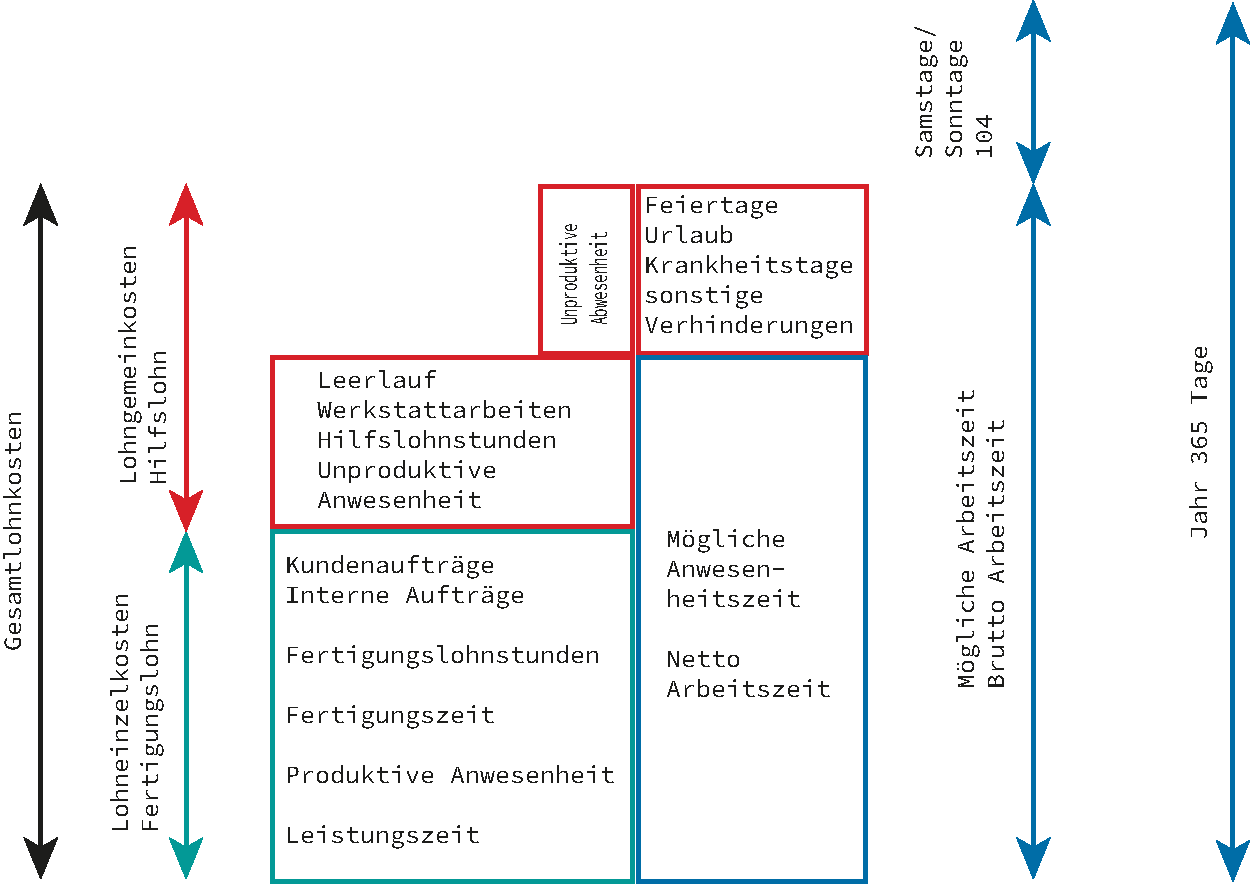
\includegraphics[width=0.9\textwidth]{images/Skizze/Arbeitszeitermittlung.pdf}
\caption{Arbeitszeitermittlung}
%\label{fig:}%% anpassen
\end{figure}

\textbf{Ermittlungsschema}

\lstset{language=Python}% C, TeX, Bash, Python 
\begin{lstlisting}[
	%caption={}, label={code:}%% anpassen
]
  Kalendertage pro Jahr                              365
- Samstag/Sonntag (5-Tage-Woche, 52 x 2)             104
= Mögliche Arbeitszeit (Brutto)                      261
- Feiertage (je Bundesland)                            9
- Urlaubstage (min. 24 Werktage)                      29
- Krankheitstage                                       8
- Schulungstage                                        6 
= Mögliche Anwesenheitstage (Netto)                  209
  Tägliche Arbeitszeit 8 h 
_____________________________________________________________
= Mögliche Anwesenheitszeit in Stunden (209 x 8 h) 1.672 h
  Leistungszeit (produktive Arbeitszeit)
  Leerlauf      (unproduktive Arbeitszeit)
_____________________________________________________________
= Arbeitstage pro Jahr (261 - Feiertage)             252 Tage
\end{lstlisting}

\textbf{Werktag} (Mo. - Sa.)

\newpage

\section{Serviceberater - Kundendienstberater -
Dialogannahme}\label{serviceberater-kundendienstberater-dialogannahme}

\textbf{Skript - Serviceberater}

\begin{itemize}
\item
  >>Mädchen für alles<<
\item
  Vollzeitjob, hat viele Einsatzmöglichkeiten
\item
  Im Durchschnitt 8 bis 14 Kunden pro Tag
\item
  Small Talk halten: Wieso, Weshalb, Warum?
\item
  Das kleine 1x1 des Serviceberaters
\end{itemize}

\textbf{Vorgehensweise des KD-Beraters bei der Auftragsannahme}

\begin{itemize}
\item
  Fragen nach dem Kundenwunsch
\item
  Durchführung der Untersuchung des Fahrzeuges
\item
  Dokumentation von Schäden am Fahrzeug
\item
  Erfassung von Wertgegenständen im Fahrzeug
\item
  Probefahrt mit dem Kunden
\item
  Mitteilung des kalkulierten Preises
\item
  Auftrag erstellen
\end{itemize}

\textbf{Vorteile Direktannahme}

\begin{itemize}
\item
  Möglichkeit zur Kommunikation mit dem Kunden schaffen
\item
  über Mängel sofort informieren
\item
  Missverständnisse können vermieden werden
\item
  Rückfragen werden verringert
\item
  teure Reparatur erkennen vs.~Zeitwert / Wiederbeschaffungswert $\to$
  zeitwertgerechte Reparatur
\item
  günstige Ersatzteile oder Gebrauchtteile $\to$ verkehrstüchtigen
  Zustand
\item
  bei sicherheitsrelevanten Mängel $\to$ nicht mehr fahren lassen!
  (Polizei informieren bei hartnäckigen Fällen)
\item
  Entscheidend ist kompetente Person oder Schnarchnase!
\end{itemize}


	%%%%%%%%%%%%%%%%%%%%%%%%%%%%%%%%%%%%%%%%%%%%%%%%%%%%%%%%%%%%%%%%%%
    % Bibliographie
    \printbibliography[category=cited]
\end{document}
